\documentclass{article}

% Paquetes comunes
\usepackage[utf8]{inputenc}
\usepackage[T1]{fontenc}
\usepackage[spanish]{babel}
\usepackage{amsmath, amssymb}
\usepackage{graphicx}
\usepackage{float}
\usepackage{geometry}
\usepackage{hyperref}
\usepackage{fancyhdr}
\usepackage{textcomp}
\usepackage{circuitikz}
% Saltar entre párrafos - sin sangrías
\usepackage{parskip}

% Márgenes
\geometry{a4paper, margin=2.5cm}

% Encabezado y pie de página
\pagestyle{fancy}
\fancyhf{}
\fancyhead[L]{\textbf{Tarea 5} - Tomas Infante}
\fancyhead[R]{IEE2513}
\fancyfoot[C]{\thepage}

\title{Tarea 5}
\author{Tomas Infante}
\date{\today}
\begin{document}
\begin{figure}[H]
    \centering
    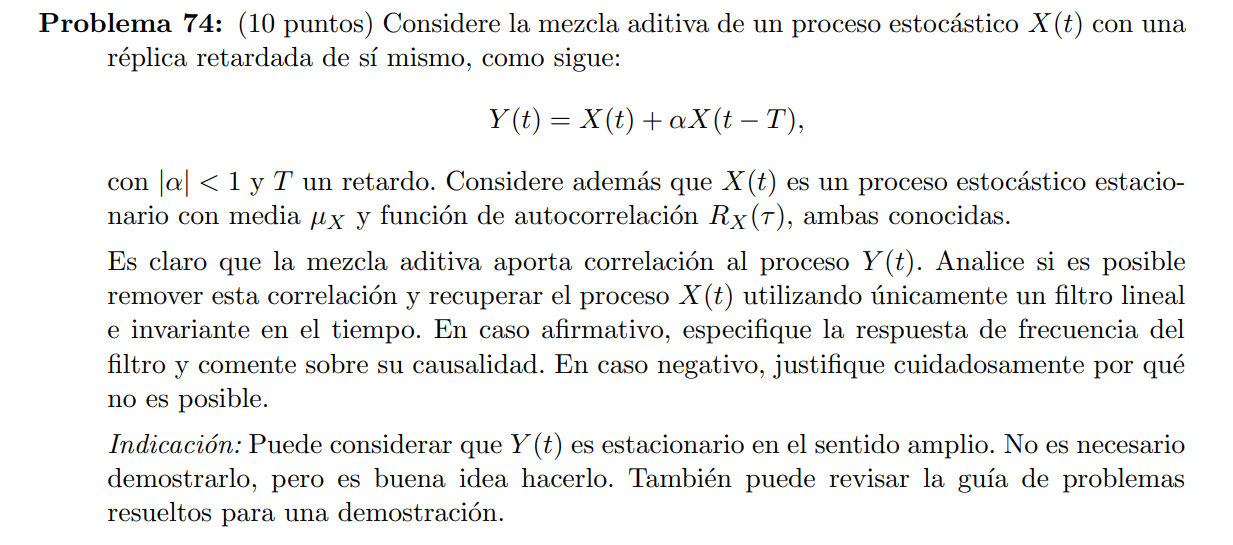
\includegraphics[width=1\textwidth]{Problema_74.png}
    \label{Problema_74}
\end{figure}
Para este problema hay que hacer un poco de ingenieria inversa, ya que podemos suponer que \(Y(t)\) es la señal de salida de un filtro por el cual pasa \(X(t)\). Ahora bien, si ese filtro existe y tiene inverso, entonces ese filtro inverso seria el que estamos buscando.\\

Podemos considerar un filtro con respuesta al impulso:
\[
h(t)= \delta(t) +\alpha \delta(t - T)
\]
Es claro que si aplicamos este filtro a \(X(t)\) y definimos \(Y(t)\) como la salida de ese filtro, entonces se cumple:
\[
Y(t)=h(t)\ast X(t)
\]
Lo que es facil de comprobar, ya que:
\[
Y(t)=\int_{-\infty}^{\infty}h(\tau)X(t-\tau)\,d\tau
\]
\[
Y(t) = \int_{-\infty}^{\infty}\left[\delta(\tau) +\alpha \delta(\tau-T)\right]X(t-\tau)\,d\tau
\]
\[
Y(t) = X(t)+\alpha X(t-T)
\]
Si analizamos el filtro en frecuencia, llegamos a que:
\[
\mathcal{F}\left\{h(t)\right\}= \mathcal{F}\left\{\delta(t) +\alpha \delta(t-T)\right\}
\]
\[
H(\omega)= 1+\alpha e^{-j\omega T}
\]
Este filtro en frecuencia describe \(Y(\omega)\) segun:
\[
Y(\omega)= H(\omega)X(\omega)
\]
Entonces necesitamos un filtro \(G(\omega)\) tal que:
\[
X(\omega)=G(\omega)Y(\omega)
\]
Si partimos de:
\[
Y(\omega)= H(\omega)X(\omega) \quad \longrightarrow \quad \frac{1}{H(\omega)}Y(\omega)=X(\omega)
\]
Es decir, existe un filtro inverso en frecuencia:
\[
G(\omega) = \frac{1}{H(\omega)} = \frac{1}{1+\alpha e^{-j\omega T}}
\]
Notemos que:
\[
|1+\alpha e^{-j\omega T}|\geq 1-|\alpha|>0
\]
ya que \(|e^{-j\omega T}|=1\). Por lo tanto:
\[
H(\omega)\neq 0 \quad \forall \omega
\]
lo que asegura que el sistema es invertible.

Como \(|\alpha|<1\), se cumple que \(|-\alpha e^{-j\omega T}|=|\alpha|<1\), por lo que se puede reescribir como una serie geometrica, ya que:
\[
\sum_{k=0}^{\infty}r^{k} = \frac{1}{1-r}\quad |r|<1
\]
Por lo tanto:
\[
\frac{1}{1+\alpha e^{-j\omega T}} = \sum_{k=0}^{\infty}(-\alpha e^{-j\omega T})^{k} = \sum_{k=0}^{\infty}(-\alpha)^{k} e^{-j\omega kT}
\]
Ahora debemos calcular la transformada inversa de \(G(\omega)\):
\[
g(t) = \mathcal{F}^{-1}\left\{G(\omega)\right\} = \sum_{k=0}^{\infty}(-\alpha)^{k} \mathcal{F}^{-1}\left\{e^{-j\omega kT}\right\} 
\]
\[
g(t) = \sum_{k=0}^{\infty}(-\alpha)^{k} \delta(t-kT)
\]
Por lo tanto, el filtro inverso existe y permite recuperar \(X(t)\) a partir de \(Y(t)\), teniendo como respuesta al impulso \(g(t)\).
\begin{figure}[H]
    \centering
    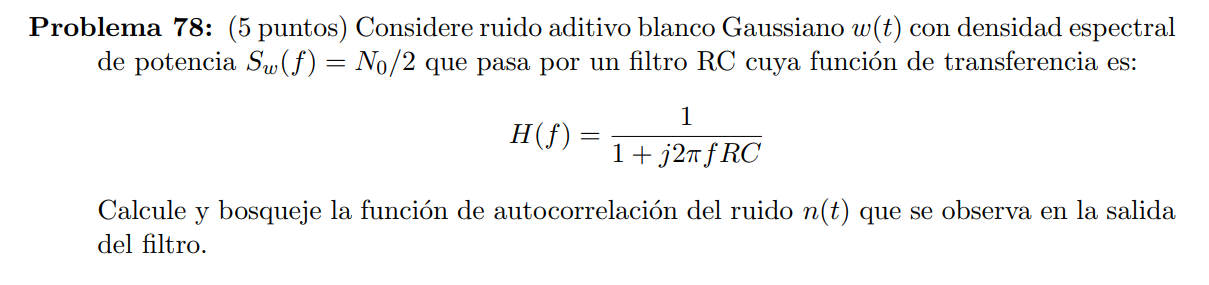
\includegraphics[width=1\textwidth]{Problema_78.png}
    \label{Problema_78}
\end{figure}
Sabemos que:
\[
S_n(f)=|H(f)|^{2}S_\omega (f)
\]
Donde:
\[
|H(f)|^{2} = \frac{1}{1+(2\pi f RC)^{2}}
\]
Por lo tanto:
\[
S_n(f)=|H(f)|^{2}S_\omega (f) = \left(\frac{1}{1+(2\pi f RC)^{2}}\right)\frac{N_0}{2}
\]
\[
S_n(f)= \frac{N_0}{2\left(1+(2\pi f RC)^{2}\right)}
\]
Para obtener la funcion de autocrrelacion debemos tener en cuenta que:
\[
\mathcal{F}^{-1}\left\{S_n(f)\right\} = R_n(\tau)
\]
Y tenemos que:
\[
\mathcal{F}^{-1}\left\{S_n(f)\right\} = \frac{N_0}{2}\mathcal{F}^{-1}\left\{\frac{1}{1+(2\pi f RC)^{2}}\right\}
\]
Noostros sabemos que:
\[
\mathcal{F}^{-1}\left\{\frac{2a}{a^{2}+(2\pi f)^{2}}\right\}=e^{-a|t|}\quad a>0
\]
Asi que tenemos que llevar la expresion que tenemos a algo similar:
\[
\frac{1}{1+(2\pi f RC)^{2}} = \frac{1}{1+(RC)^{2}(2\pi f)^{2}}= \frac{1}{(RC)^{2}\left[\frac{1}{(RC)^{2}}+(2\pi f)^{2}\right]}
\]
\[
\frac{1}{1+(2\pi f RC)^{2}} = \frac{1}{2RC}\left[\frac{\frac{2}{RC}}{\frac{1}{(RC)^{2}}+(2\pi f)^{2}}\right]
\]
Por lo tanto:
\[
\mathcal{F}^{-1}\left\{\frac{1}{1+(2\pi f RC)^{2}}\right\} = \mathcal{F}^{-1}\left\{\frac{1}{2RC}\left[\frac{\frac{2}{RC}}{\frac{1}{(RC)^{2}}+(2\pi f)^{2}}\right]\right\}
\]
\[
= \frac{1}{2RC} \mathcal{F}^{-1}\left\{\left[\frac{\frac{2}{RC}}{\frac{1}{(RC)^{2}}+(2\pi f)^{2}}\right]\right\} \qquad a = \frac{1}{RC}
\]
\[
\mathcal{F}^{-1}\left\{\frac{1}{1+(2\pi f RC)^{2}}\right\} = \frac{1}{2RC}e^{-\frac{|t|}{RC}}
\]
Entonces:
\[
\mathcal{F}^{-1}\left\{S_n(f)\right\} = \frac{N_0}{2}\mathcal{F}^{-1}\left\{\frac{1}{1+(2\pi f RC)^{2}}\right\}
\]
\[
\mathcal{F}^{-1}\left\{S_n(f)\right\} = \frac{N_0}{2}\frac{1}{2RC}e^{-\frac{|t|}{RC}}
\]
\[
R_n(\tau) = \frac{N_0}{4RC}e^{\frac{|\tau|}{RC}}
\]
\begin{figure}[H]
    \centering
    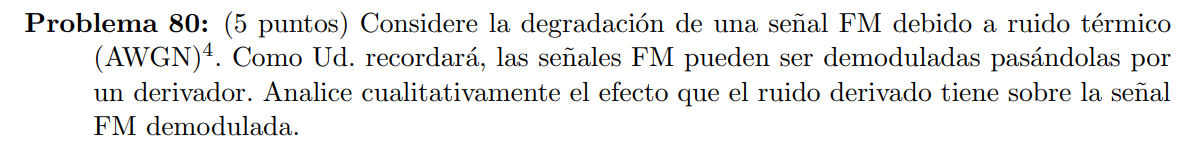
\includegraphics[width=1\textwidth]{Problema_80.png}
    \label{Problema_80}
\end{figure}
Para analizar el efecto del ruido termico en una señal FM, recordemos que la demodulacion FM puede realizarse derivando la señal recibida. Si la señal recibida es:

\[
r(t)=s(t)+w(t)
\]

donde \(s(t)\) es la señal FM y \(w(t)\) es ruido blanco Gaussiano, entonces al derivar se obtiene:

\[
\frac{d}{dt}r(t)=\frac{d}{dt}s(t)+\frac{d}{dt}w(t)
\]

Es decir, tanto la señal como el ruido pasan por un derivador.

En frecuencia, derivar equivale a multiplicar por \(j2\pi f\), por lo que el modulo del sistema es:

\[
|H(f)|=2\pi |f|
\]

Esto muestra que las componentes de mayor frecuencia se amplifican mas que las de baja frecuencia.

Como el ruido blanco tiene energia en todas las frecuencias, al pasar por el derivador sus componentes de alta frecuencia se amplifican fuertemente. Por otro lado, la señal FM contiene la informacion en la variacion de frecuencia, por lo que el derivador permite recuperar la señal deseada.

Sin embargo, el efecto sobre el ruido es importante: despues de la derivacion, el ruido deja de ser uniforme en frecuencia y pasa a estar dominado por las componentes de alta frecuencia. Esto implica que la señal demodulada queda contaminada principalmente por ruido en altas frecuencias.

En conclusion, el proceso de derivacion necesario para demodular FM empeora el efecto del ruido termico, ya que amplifica fuertemente sus componentes de alta frecuencia, lo que degrada la calidad de la señal demodulada.

\end{document}